%\tableofcontents
\chapter{Multi-orbital extension of FLEX self-energy}
\label{chap:MO_FLEX}
\section{Introduction}

An accurate description of the electronic structure of correlated materials has yet to be developed in equilibrium. 
Generally, in strongly correlated materials, several orbitals are falling into the low-energy region around the Fermi level. A description of these materials requires an extension of the Hubbard model to the multiorbital one. Even in high-$T_c$ cuprates, where orbitals other than the one that forms the Fermi surface are neglected in many cases, the orbital degrees of freedom play an essential role \citep{PhysRevLett.105.057003, PhysRevB.85.064501, PhysRevB.87.045113}.

The multiorbital FLEX approach has already been applied to iron and nickel in self-consistent and non-self-consistent forms in equilibrium. In this chapter, we write about multiorbital DMFT+FLEX and DMFT+PP based on real-time Keldysh contour technic which later on gives the possibility to investigate nonequilibrium effects. We use the Hubbard model in a paramagnetic state with density-density type interaction and degenerate orbitals \citep{2005JPCM...17...61D}. Multiorbital time-independent Hamiltonian has a form
\begin{subequations}
\begin{align}
H
&=
	\sum_{{\bf{R}} \lambda,\bf{R}' \lambda'}{t_{{\bf{R}} \lambda,{\bf{R}}' \lambda'} c_{\bf{R} \lambda}^{\dagger} c_{{\bf{R}}' \lambda'}} 
		\nonumber
		\\
 &+
1/2 \sum_{{\bf{R}},\lambda,\lambda',\lambda'',\lambda'''}{\langle {\bf{R}} \lambda, {\bf{R}} \lambda' \vert V \vert \langle {\bf{R}} \lambda'', {\bf{R}} \lambda''' \rangle c_{{\bf{R}},\lambda}^{\dagger} c_{{\bf{R}},\lambda'}^{\dagger} c_{{\bf{R}},\lambda'''} c_{{\bf{R}},\lambda''}}
\end{align}
\end{subequations}
where ${\bf{R}}$ is lattice site coordinates and $\lambda = (l\sigma)$ is spin-orbital indices. The hopping term $t_{{\bf{R}} \lambda,{\bf{R}}' \lambda'}$ is determined from ab-initio electronic structure calculations and will be replaced in this comparison study with a model dispersion relation diagonal in the spin-orbital indices. The electron interaction is usually considered only between the $d$ electrons, since the effect of the lower orbitals is assumed to be described well with the density functional theory (DFT) technic. The interaction was taken in the form of a Kanamori matrix.
\FloatBarrier
\section{FLEX self-energy}
\label{section:FLEX_self_energy}
The effects of the electron interaction on one-particle states are described by the self-energy $\Sigma$:
\begin{equation}
\Sigma_{\lambda}^{FLEX}(t,t')= \Sigma_{\lambda}^{HF}(t,t')\delta(t,t')-2\Sigma_{\lambda}^{2}(t,t') + \Sigma_{\lambda}^{PH}(t,t') + \Sigma_{\lambda}^{PP}(t,t')+ \Sigma_{\lambda}^{INT}(t,t')
\end{equation}
where self energies: $\Sigma^{HF}(t,t')$ - Hartree-Fock, $\Sigma^{2}(t,t')$ - second order perturbation theory, $\Sigma^{PH}(t,t')$ - particle-hole, $\Sigma^{PP}(t,t')$ - particle-particle, $\Sigma^{int}(t,t')$ - "interaction" self energy.


\begin{equation}
\Sigma_{\lambda}^{HF}(t)=\sum_{\lambda'}U_{\lambda \lambda'}(t)n_{\lambda'}(t)\delta(t,t')
\end{equation}
where $n$ -number of particle

The simplest approximation to the vertex function for the self energy is the bare interaction $U_{\lambda \lambda'}$. Such
an approximation corresponds to second-order perturbation theory (SOPT).
\begin{equation}
\Sigma_{\lambda}^{2}(t,t')=-i\sum_{\lambda'}U(t)\chi_{\lambda \lambda'}^{PH0}(t,t')U(t')G_{\lambda'}(t,t')
\end{equation}
where electron-hole polarisation bubble is
\begin{equation}
\chi_{\lambda \lambda'}^{PH0}(t,t')=iG_{\lambda}(t,t')G_{\lambda'}(t',t)
\end{equation}

Full particle-hole self energy:
This chahhal can be separeted into particle-hole and interaction parts:
\begin{equation}
\Sigma_{\lambda}^{PH}(t,t')=-i\sum_{\lambda'}V_{\lambda \lambda'}(t,t')G_{\lambda'}(t,t')
\end{equation}
\begin{equation}
V_{\lambda \lambda'}^{PH}(t,t')=U_{\lambda \lambda'}(t) \chi_{\lambda \lambda'}^{PH}(t,t')U_{\lambda \lambda'}(t')
\end{equation}

When we sum ladder particle-hole diagrams we obtain for the vertex function:
\begin{equation}
\chi_{\lambda \lambda'}^{PH}(t,t')=\chi_{\lambda \lambda'}^{PH0}(t,t')+\int_C{\chi_{\lambda \lambda'}^{PH0}(t,t_1)U(t_1)\chi_{\lambda \lambda'}^{PH}(t_1,t') dt_1}
\end{equation}

Two-particle scatterings is the interaction channel:
\begin{equation}
\Sigma_{\lambda}^{INT}(t,t')=i G_{\lambda}(t,t') V_{\lambda \lambda}^{INT}(t,t')
\end{equation}
\begin{equation}
V_{\lambda \lambda}^{INT}(t,t')=U_{\lambda \lambda}(t) \chi_{\lambda \lambda}^{INT}(t,t')U_{\lambda \lambda}(t')
\end{equation}
\begin{equation}
\chi_{\lambda \lambda}^{INT}(t,t')=\chi_{\lambda \lambda}^{INT0}(t,t')+\int_C{\chi_{\lambda \lambda}^{INT0}(t,t_1)U(t_1)\chi_{\lambda \lambda}^{INT}(t_1,t') dt_1}
\end{equation}
\begin{equation}
\begin{split}
&{\chi_{\lambda \lambda'}^{PH_{int}0}(t,t')=0 \; \; if \; \; \lambda \ne \lambda'};\\
&{\chi_{\lambda \lambda'}^{PH_{int}0}(t,t')=\chi_{\lambda \lambda}^{PH_{int}0}(t,t')=-iG_{\lambda}(t,t')G_{\lambda}(t',t) \; \; if \; \; \lambda=\lambda'}.
\end{split}
\end{equation}

Analogously we can construct an approximation with multiple electron-electron scatterings where the self-energy can be represented as:
\begin{equation}
\Sigma_{\lambda}^{PP}(t,t')=-i\sum_{\lambda'}V_{\lambda \lambda'}^{PP}(t,t')G_{\lambda'}(t',t)
\end{equation}
\begin{equation}
V_{\lambda \lambda'}^{PP}(t,t')=U_{\lambda \lambda'}(t) \chi_{\lambda \lambda'}^{PP}(t,t')U_{\lambda \lambda'}(t')
\end{equation}
\begin{equation}
\chi_{\lambda \lambda'}^{PP}(t,t')=\chi_{\lambda \lambda'}^{PP0}(t,t')+\int_C{\chi_{\lambda \lambda'}^{PP0}(t,t_1)U(t_1)\chi_{\lambda \lambda'}^{PP}(t_1,t') dt_1}
\end{equation}
where particle-particle polarisation bubble is
\begin{equation}
\chi_{\lambda \lambda'}^{PP0}(t,t')=iG_{\lambda}(t,t')G_{\lambda'}(t,t')
\end{equation}

We can treat each channel independently or add all three to assess the effect of dynamical fluctuations on the electron self-energy.
In the latter case, however, we have to subtract twice the contribution from the second-order, since it is identical in all three channels.

It is known that FLEX has a divergence in the particle-hole channel. To get rid of this divergence, we introduce a screened interaction ($U_{scr}$), which we use instead of $U$ in particle-hole and interaction channels. $U_{scr}$ was calculated in imaginary and real-time using particle-particle channel \citep{PhysRevB.72.115106,PhysRevB.92.195123,PhysRevLett.114.246402}.

\FloatBarrier

\section{Equilibrium multi-orbital Hubbard model}
\label{section:E_mb_Hubbard_model}
Calculations were performed on infinitely dimensional Bethe lattice with semi-elliptic density of states $\rho_0(E)={2 \over \pi}\sqrt{1-E^{2}}$.
We tested electron-hole and electron-electron channels. DMFT type of self-consistency used in this work. All approximations were calculated in real-time in Keldysh contour.

We calculated the analytical approximations for small to an intermediate value of the interaction strength. All energies are given in units of the half-bandwidth of the non-interacting DOS, $D = 1$. In calculation used 2000 points in Matsubara branch of the contour, up to 3000 points in real-time color with $h=0.02$ time-step, inverse temperature $\lambda'=16$, the error value of DMFT convergence is $1\times10^{-10}$.

In Fig.~\ref{fig:2_orb_DOS_pp_mu0_eq}a is shown interaction dependece of two-orbital DOS calculated with particle-particle self energy (DMFT+PP) in half-filling and corresponding self energy Fig.~\ref{fig:2_orb_Sigma_pp_mu0_eq}a. In DOS is seen tendension to formation Hubbard bands with increasing Coulomb interaction. Spectral function for $U=2$ has Hubbard bands located in -2 and 2 in energy axis, this result is consistent with work \citet{2005JPCM...17...61D}. Dependence of relarion $J_H/U=q$ for $U=2$ presented in Fig.~\ref{fig:2_orb_DOS_pp_mu0_eq}b for DOS and Fig.~\ref{fig:2_orb_Sigma_pp_mu0_eq}b self energy. Increasing $q$ Hubbard bands decreases with saving thairs positions. 
\begin{figure}[h!]
\begin{minipage}[h]{0.5\linewidth}
\center{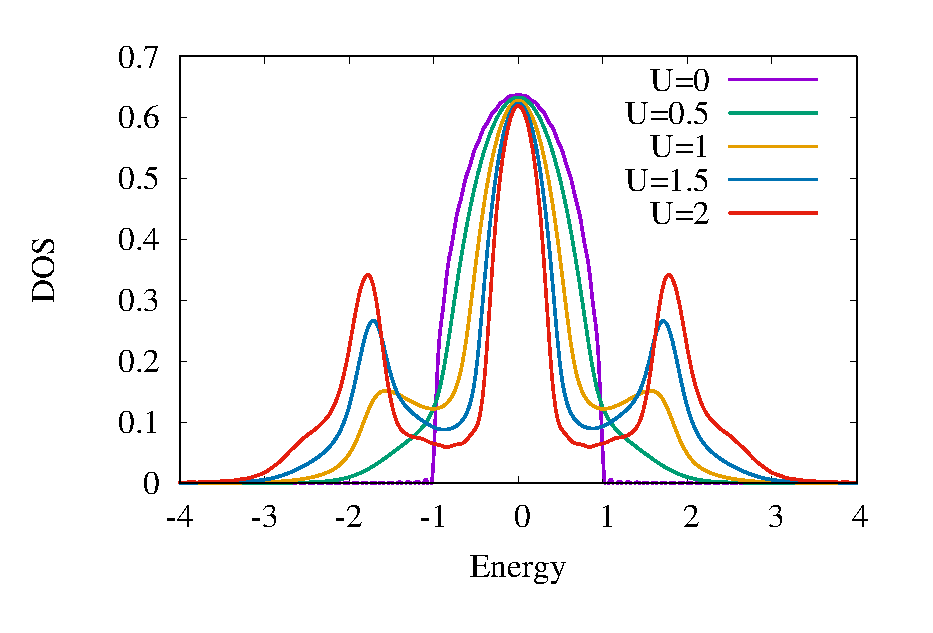
\includegraphics[width=1\linewidth]{Chapters/2orb_DMFT/figure/pp/DOS_mu0_J0.eps}} (a) \\
\end{minipage}
\hfill
\begin{minipage}[h]{0.5\linewidth}
\center{\includegraphics[width=1\linewidth]{Chapters/2orb_DMFT/figure/pp/DOS_mu0_J.eps}} (b) \\
\end{minipage}
\caption{DOS two-orbital DMFT+PP $n=0.5$ (half-filled): (a) Interaction dependence with $J_{H}=0$, (b) $q$-dependence with fixed $U=2$.}
\label{fig:2_orb_DOS_pp_mu0_eq}
\end{figure}

\begin{figure}[h!]
\begin{minipage}[h]{0.5\linewidth}
\center{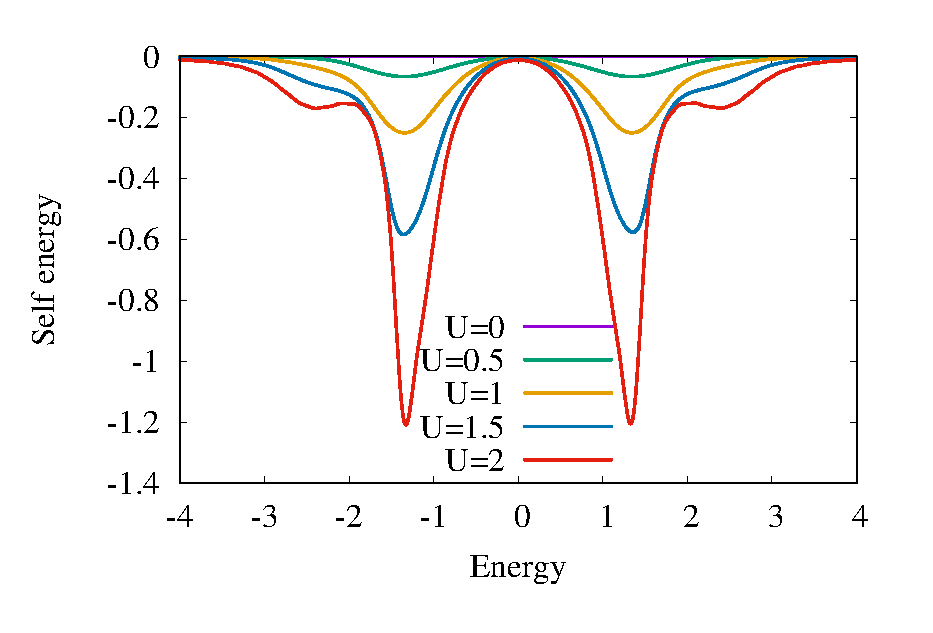
\includegraphics[width=1\linewidth]{Chapters/2orb_DMFT/figure/pp/Sigma_mu0_J0.eps}} (a) \\
\end{minipage}
\hfill
\begin{minipage}[h]{0.5\linewidth}
\center{\includegraphics[width=1\linewidth]{Chapters/2orb_DMFT/figure/pp/Sigma_mu0_J.eps}} (b) \\
\end{minipage}

\caption{Self energy two-orbital DMFT+PP $n=0.5$ (half-filled): (a) Interaction dependence with $J_{H}=0$, (b) $q$-dependence with fixed $U=2$.}
\label{fig:2_orb_Sigma_pp_mu0_eq}
\end{figure}

Fig.~\ref{fig:2_orb_DOS_pp_mu_eq} demonstrates DOS with partially filled band calculated using particle-particle self energy. The density of states has a broad peak in zero energy and creates another slim peak in the side of positive energies. This high energy peak reacted for changing Coulomb interaction or relation of interaction to Hund coupling $q$, while the low-energy peak almost does not change. Self energies for this cases are shown in Fig.~\ref{fig:2_orb_Sigma_pp_mu_eq}.
\begin{figure}[h!]
\begin{minipage}[h]{0.5\linewidth}
\center{\includegraphics[width=1\linewidth]{Chapters/2orb_DMFT/figure/pp/DOS_mu_J0.eps}} (a) \\
\end{minipage}
\hfill
\begin{minipage}[h]{0.5\linewidth}
\center{\includegraphics[width=1\linewidth]{Chapters/2orb_DMFT/figure/pp/DOS_mu_J.eps}} (b) \\
\end{minipage}
\caption{DOS two-orbital DMFT+PP $n=0.2$: (a) Interaction dependence with $J_{H}=0$, (b) $q$-dependence with fixed $U=1.8$.}
\label{fig:2_orb_DOS_pp_mu_eq}
\end{figure}


\begin{figure}[h!]
\begin{minipage}[h]{0.5\linewidth}
\center{\includegraphics[width=1\linewidth]{Chapters/2orb_DMFT/figure/pp/Sigma_mu_J0.eps}} (a) \\
\end{minipage}
\hfill
\begin{minipage}[h]{0.5\linewidth}
\center{\includegraphics[width=1\linewidth]{Chapters/2orb_DMFT/figure/pp/Sigma_mu_J.eps}} (b) \\
\end{minipage}
\caption{Self energy two-orbital DMFT+PP $n=0.2$: (a) Interaction dependence with $J_{H}=0$, (b) $q$-dependence with fixed $U=1.8$.}
\label{fig:2_orb_Sigma_pp_mu_eq}
\end{figure}

In Fig.~\ref{fig:2_orb_DOS_FLEX_mu0_eq}a is shown interaction dependence of two-orbital DOS calculated with FLEX self energy (DMFT+FLEX) in half-filling. DOS has a trend in the formation of Hubbard bands with increasing Coulomb interaction. Hubbard peaks less pronounced compared to particle-particle self-energy case. Also it is seen the formation of low energy shoulders with increasing $U$ in quasiparticle peak. Dependence of $q$ for $U=1.5$ presented in Fig.~\ref{fig:2_orb_DOS_FLEX_mu0_eq}b for DOS and Fig.~\ref{fig:2_orb_Sigma_pp_mu0_eq}b for self energy. Increasing $q$ Hubbard bands decreases. 
\begin{figure}[h!]
\begin{minipage}[h]{0.5\linewidth}
\center{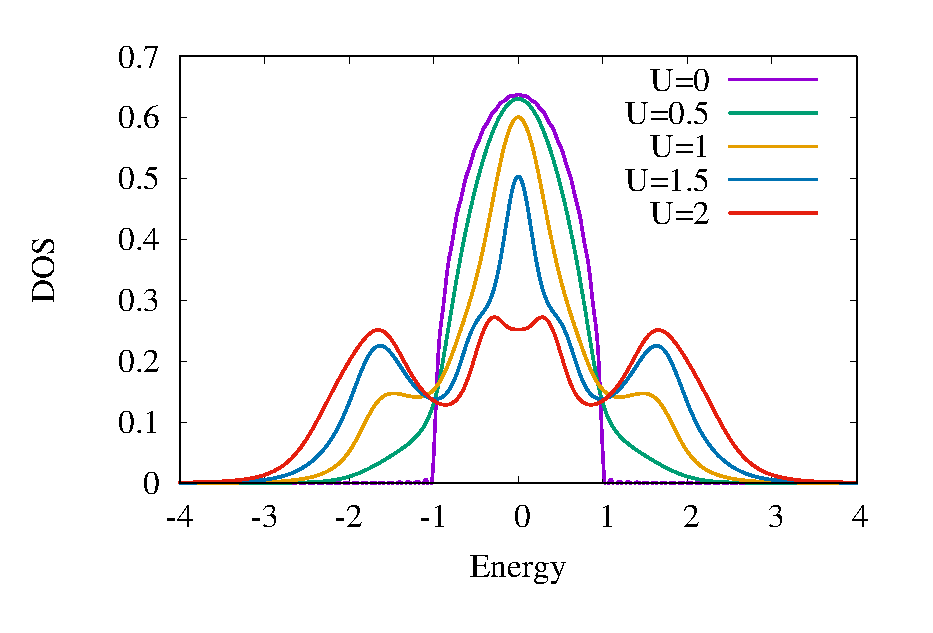
\includegraphics[width=1\linewidth]{Chapters/2orb_DMFT/figure/FLEX/DOS_mu0_J0.eps}} (a) \\
\end{minipage}
\hfill
\begin{minipage}[h]{0.5\linewidth}
\center{\includegraphics[width=1\linewidth]{Chapters/2orb_DMFT/figure/FLEX/DOS_mu0_J.eps}} (b) \\
\end{minipage}
\caption{DOS of two-orbital DMFT+FLEX $n=0.5$ (half-filled): (a) Interaction dependence with $J_{H}=0$, (b) $q$-dependence with fixed $U=1.8$.}
\label{fig:2_orb_DOS_FLEX_mu0_eq}
\end{figure}

Self-energy (Fig.~\ref{fig:2_orb_Sigma_FLEX_mu0_eq}a) has a significantly different shape and has a positive value in zero energy in comparison with particle-particle self-energy. 
\begin{figure}[h!]
\begin{minipage}[h]{0.5\linewidth}
\center{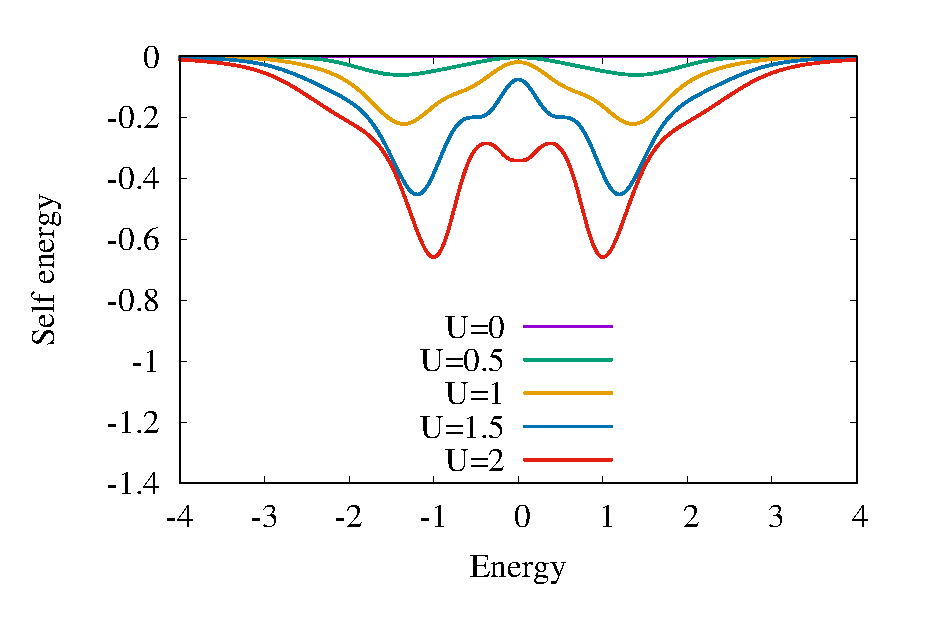
\includegraphics[width=1\linewidth]{Chapters/2orb_DMFT/figure/FLEX/Sigma_mu0_J0.eps}} (a) \\
\end{minipage}
\hfill
\begin{minipage}[h]{0.5\linewidth}
\center{\includegraphics[width=1\linewidth]{Chapters/2orb_DMFT/figure/FLEX/Sigma_mu0_J.eps}} (b) \\
\end{minipage}
\caption{Self-energy of two-orbital DMFT+FLEX $n=0.5$ (half-filled): (a) Interaction dependence with $J_{H}=0$, (b) $q$-dependence with fixed $U=1.5$.}
\label{fig:2_orb_Sigma_FLEX_mu0_eq}
\end{figure}

\begin{figure}[h!]
\begin{minipage}[h]{0.5\linewidth}
\center{\includegraphics[width=1\linewidth]{Chapters/2orb_DMFT/figure/FLEX/DOS_mu_J0.eps}} (a) \\
\end{minipage}
\hfill
\begin{minipage}[h]{0.5\linewidth}
\center{\includegraphics[width=1\linewidth]{Chapters/2orb_DMFT/figure/FLEX/DOS_mu_J.eps}} (b) \\
\end{minipage}
\caption{DOS of two-orbital DMFT+FLEX $n=0.2$: (a) Interaction dependence with $J_{H}=0$, (b) $q$-dependence with fixed $U=1.6$.}
\label{fig:2_orb_DOS_FLEX_mu_eq}
\end{figure}

\begin{figure}[h!]
\begin{minipage}[h]{0.5\linewidth}
\center{\includegraphics[width=1\linewidth]{Chapters/2orb_DMFT/figure/FLEX/Sigma_mu_J0.eps}} (a) \\
\end{minipage}
\hfill
\begin{minipage}[h]{0.5\linewidth}
\center{\includegraphics[width=1\linewidth]{Chapters/2orb_DMFT/figure/FLEX/Sigma_mu_J.eps}} (b) \\
\end{minipage}
\caption{Self-energy two-orbital DMFT+FLEX $n=0.2$: (a) Interaction dependence with $J_{H}=0$, (b) $q$-dependence with fixed $U=1.6$.}
\label{fig:2_orb_Sigma_FLEX_mu_eq}
\end{figure}

Fig.~\ref{fig:2_orb_DOS_FLEX_mu_eq} demonstrates DOS for partially filled band calculated using FLEX self energy. The density of states has a broad peak in zero energy and a second slim peak in the side of positive energies. This high energy peak reacted for changing Coulomb interaction or relation of interaction to Hund coupling $q$, while the low-energy peak almost does not change. FLEX self energies shown in Fig.~\ref{fig:2_orb_Sigma_FLEX_mu_eq}. Thus, the behavior of DOS and self-energy in FLEX and PP are similar. PP cases have slightly bigger amplitudes.

In Fig.~\ref{fig:2_orb_Z_u} is depicted quasiparticle weight ($Z$) as function on Couloumb interaction. $Z$ was calculated using formula:
\begin{equation}
Z={\left( \left. 1-{\partial Re \Sigma(\omega) \over \partial \omega}\right|_{\omega \to 0}\right)}^{-1}
\end{equation}

There are lines correspond to different self-energy contributions using in DMFT scheme: red - second-order perturbation theory (SOPT), blue - particle-particle channel, FLEX${_0}$ - fluctuation exchange approximation without interaction channel, purple - full FLEX, black line - QMC data obtain from \citep{2005JPCM...17...61D}. Comparison of data with QMC result it is seen that SOPT work good in regime with small interaction until $U=1.7$ and further underestimate $Z$, PP stable during all considered interaction and overestimate $Z$, which does not agree with \citep{2005JPCM...17...61D}. FLEX$_0$ and FLEX have relatively good agreement with QMC data until $U$=1.7 and after $Z$ drastically increases.
\begin{figure}[h!]
\center{\includegraphics[width=0.8\linewidth]{Chapters/2orb_DMFT/figure/Z.eps}} 
\caption{Quasiparticle weight as function of Coulomb interaction for DMFT with different contribution in self energy.}
\label{fig:2_orb_Z_u}
\end{figure}

In the Fig.~\ref{fig:2_orb_Z_u_J} is shown the results for quasiparticle weight as a function of Coulomb interaction for FLEX self-energy with different Hund coupling. FLEX self-energy was chosen because it gives the best overlap with QMC data. Fig.~\ref{fig:2_orb_Z_u_J}a represents data for $q$-dependence with $n=0.5$, the higher Hund coupling (or $q$ relation) then bigger $Z$ for considered $U$. Such growth of $Z$ occurs until $q=0.2$, $q=0.3$ repeated results of the previous $q$ at least in small $U$ range.

Similar result occur for $q$-dependence with $n=0.25$ Fig.~\ref{fig:2_orb_Z_u_J}b and rising of $Z$ till $q=0.3$. 

In comparing these two graphs seen that in general doping of the system raises $Z$.
\begin{figure}[h!]
\begin{minipage}[h]{0.5\linewidth}
\center{\includegraphics[width=1\linewidth]{Chapters/2orb_DMFT/figure/Z_J.eps}} (a) \\
\end{minipage}
\hfill
\begin{minipage}[h]{0.5\linewidth}
\center{\includegraphics[width=1\linewidth]{Chapters/2orb_DMFT/figure/Z_J_n025.eps}} (b) \\
\end{minipage}
\caption{Quasiparticle weight as function of Coulomb interaction for FLEX self energy: (a) $q$-dependence with $n=0.5$, (b) $q$-dependence with $n=0.25$.}
\label{fig:2_orb_Z_u_J}
\end{figure}

Thus, we considered paramagnetic two degenerate orbitals with the density-density type interaction Hubbard model. This model has significant advantages: simple to implement, extremely cheap in computational resources compare to other multiorbital models and gives reasonable results in certain parameter ranges. Disadvantages: for all considered types of self-energies, it overestimates positions of Hubbard peaks. It is known that with an increase in the number of orbitals, the results deteriorate.
\FloatBarrier

%\section{Benchmark of nonequilibrium multiorbital Hubbard model}

%In equilibrium, considered above DMFT+FLEX with $J_H=0$ and $n$=0.5 give good agreement in $Z$ with exact method for $U \in $ 0-1.7. Thus consider the model in the nonequilibrium regime. For that, we apply a short pulse of the electric field. We describe the external spatially uniform electric field via the vector potential $A(t)$. The Peierls substitution is used to account for the electric field in the Hamiltonian.
%\begin{figure}[h!]
%\begin{minipage}[h]{0.5\linewidth}
%\center{\includegraphics[width=1\linewidth]{Chapters/2orb_DMFT/figure/scr_U_A3.eps}} (a) \\
%\end{minipage}
%\hfill
%\begin{minipage}[h]{0.5\linewidth}
%\center{\includegraphics[width=1\linewidth]{Chapters/2orb_DMFT/figure/E_tot_A3.eps}} (b) %\\
%\end{minipage}
%\caption{Nonequilibrium behavior in the presence of short electric pulse: (a) screened interaction, (b) total energy.}
%\label{fig:2_orb_Benchmark}
%\end{figure}

%Results of screened interaction and total energy shown in Fig.~\ref{fig:2_orb_Benchmark}. Monocycle vector potential limited by Gaussian envelope has a maximum value of $A_{max}$=1.76. Field starts at $time_{start}$=0 and ends at $time_{end}$=1.125. A black horizontal dot-line shows pulse end in Fig.~\ref{fig:2_orb_Benchmark}. 

%In Fig.~\ref{fig:2_orb_Benchmark}a it is seen that screened interaction drastically changes during and after the pulse. This behavior has a tendency to increase with increasing Coulomb interaction.

%Modification of total energy after pulse shows us the mode in which the method works. When field absent total energy shouldn't change because there are no energy removal mechanisms. Total energy Fig.~\ref{fig:2_orb_Benchmark}b has peak in positions of maximum amplitude of vector potential during and changing after the pulse with increasing $U$.

%From Fig.~\ref{fig:2_orb_Benchmark} it is seen that this model can be analyzed with such a pulse in a small $U<0.5$ regime where the oscillation of total energy after the pulse is too little. As well $U$-quench can be used in $\Delta U=U-U_0 \sim 0.2$. Of course, this small available for work diapason of interaction can be increased if one would use not so sharp pulse as presented as an example here or making a ramp of field and ramp of $U$ for investigations of nonequilibrium dynamics of multiorbital Hubbard model.

\FloatBarrier

\section{Multi-orbital Hubbard model with full rotationally invariant Hamiltonian}
\label{section:Mb_Hubbard_frH}
The logical extension of the model, which was considered in the previous section, is avoiding degenerate model and density-density type interaction. This work was done in equilibrium for materials containing correlate $d$ or $f$ electrons using local approximation \citep{PhysRevB.57.6884}. In this section, we derive these equations in a time-dependent way.

Such Hamiltonian for the Hubbard model is:
\begin{equation}
H = H_t + H_U
%\sum^3_{i,\lambda=1} U n_{i\lambda\uparrow} n_{i\lambda\downarrow} +
% \sum_{i,\lambda\neq\lambda'} \sum_{\sigma\sigma'}
%(V-J\delta_{\sigma\sigma'})n_{i\lambda\sigma} n_{i\lambda'\sigma'}\,,
\end{equation}

Kinetic part:
\begin{equation}
H_t = \sum_{1,2,\sigma} t_{12}c^{\dagger}_{1\sigma} c_{2\sigma}
\end{equation}
where numbers=$im$ is a combination of index for site number ($i$) and the orbital ($m$).

Interaction part is:
\begin{equation}
H_U = \frac{1}{2} \sum_{1,2,3,4,\sigma,\sigma'} U_{1234}c^{\dagger}_{1\sigma} c^{\dagger}_{2\sigma'} c_{4\sigma'} c_{3\sigma}
\end{equation}

Coulomb interaction matrix defined in the following way:
\begin{equation}
U_{1234} = \int dr dr' \psi^*_{1}(r) \psi^*_{2}(r') u (r-r') \psi_{3}(r) \psi_{4}(r') 
\end{equation}
where $ u (r-r')$ - Coulomb interactions, $\psi^*_{n}(r)$ - localized on-site basis functions.


%Where $\Sigma^{TH}$ and $\Sigma^{TF}$ are the Hartree and Fock diagrams with the bare interaction replaced by the T matrix and $\Sigma^{PH}$ is the particle-hole contribution. 
First symmetrize the bare coulomb interaction over different fluctuation channels: the particle-hole (density - $U^d$ and magnetic - $U^m$) and particle-particle (singlet $U^s$ and triplet $U^t$) vertex matrices:

\begin{equation}
{\tilde{U}}_{1234} = U_{1324}
\end{equation}

\begin{equation}
U^d_{1234} = 2U_{1324}-U_{1342}
\end{equation}

\begin{equation}
U^m_{1234} = -U_{1342}
\end{equation}
  
\begin{equation}
U^s_{1234} = \frac{1}{2}[U_{1243}+U_{1234}]
\end{equation}

\begin{equation}
U^t_{1234} = \frac{1}{2}[U_{1243}-U_{1234}]
\end{equation}

For the Coulomb energy parameterization corresponds to the following matrix elements:
\begin{equation}
U_{1234} = U \quad if (1=2=3=4)
\end{equation}

\begin{equation}
U_{1234} = U' \quad if (1=3\neq2=4)
\end{equation}

\begin{equation}
U_{1234} = J_H \quad if (1=2\neq3=4)
\end{equation}

\begin{equation}
U_{1234} = J_H \quad if (1=4\neq2=3)
\end{equation}

For fully rotationally invariant Hamiltonian we assume $U' = U - 2 J_H$. Now the interaction matrix for different channels are
\[
 U =
 \begin{bmatrix}
  U & 0 & 0 & J_H \\
  0 & U-2J_H & J_H & 0 \\
  0 & J_H & U-2J_H & 0 \\
  J_H & 0 & 0 & U 
 \end{bmatrix}
\]


\[
 U^d =
 \begin{bmatrix}
  U & 0 & 0 & 2U-5J_H \\
  0 & J_H & 4J_H-U & 0 \\
  0 & 4J_H-U & J_H & 0 \\
  2U-5J_H & 0 & 0 & U 
 \end{bmatrix}
\]

\[
 U^m =
 \begin{bmatrix}
  -U & 0 & 0 & -J_H \\
  0 & -J_H & -U+2J_H & 0 \\
  0 & -U+2J_H & -J_H & 0 \\
  -J_H & 0 & 0 & -U
 \end{bmatrix}
\]


\[
 U^t =
 \begin{bmatrix}
  0 & 0 & 0 & 0 \\
  0 & \frac{3J_H-U}{2} & \frac{U-3J_H}{2} & 0 \\
  0 & \frac{U-3J_H}{2} & \frac{3J_H-U}{2} & 0 \\
  0 & 0 & 0 & 0
 \end{bmatrix}
\]



We use the following definition of for component of Green's function,
\begin{equation}
G_{12}(t,t') = -i <T_C c_1(t) c^{\dagger}_2(t')>
\end{equation}

\vspace*{0.2cm}
{\bf Calculation of Hartree-Fock self-energy ($\Sigma^{HF}$)}:

The Hartree-Fock self-energy can be written as 
\begin{equation}
\Sigma^{HF}_{12}(t,t') \delta(t,t') = U^d*n = \sum_{34} U^d_{1234}n_{34} 
\end{equation}
where * means matrix multiplication, $n$ - occupation matrix.

%\begin{equation}
%\Sigma^{TF}(t,t') = -{\large[}-i \sum_{34} T_{1432}(t,t') G_{34}(t',t){\large]} 
%\end{equation}

%The definition of components of Green's function is 

%\begin{equation}
%G_{12}(t,t') = -i <T_C c_1(t) c^{\dagger}_2(t')>
%\end{equation}

%The renormalized potential(T) in equations 6 and 7 is given by 

%\begin{equation}
%T_{1234} = U + U \star \pi^{pp} \star T
%\end{equation}

%Where $\star$ signifies the matrix product and U(t,t')= U $\delta$(t,t'). 
%In the above equation $\pi^{pp}$ is given by
\vspace*{0.2cm}
{\bf Calculation of second order self-energy ($\Sigma^{2}$)}:

The second order self-energy written as 
\begin{equation}
\Sigma^{2}_{12}(t,t') = i \sum_{34} V_{1342}(t,t') G_{34} (t,t') 
\end{equation}

Where V matrix is given by 
\begin{equation}
V_{1234}(t,t') = \sum_{5678} \tilde{U}_{1256}(t) \chi^{0,ph}_{5678} (t,t') U^d_{7834} (t') 
\end{equation}

The second-order potential for the nonmagnetic case is
\begin{equation}
V(t,t') = \tilde{U}(t)*\chi^{0,ph}(t,t')*U^d(t') %i \sum_{34} V_{1342}(t,t') G_{34} (t,t') 
\end{equation}

Where particle-hole bubble susceptibility:
\begin{equation}
\chi^{0,ph}_{1234}(t,t') = -i G_{41}(t',t) G_{23}(t,t')
\end{equation}

\vspace*{0.2cm}
{\bf Calculation of particle-hole channel of self-energy ($\Sigma^{PH}$)}:

The particle-hole channel of self-energy written as 
\begin{equation}
\Sigma^{PH}_{12}(t,t') = i \sum_{34} V^{PH}_{1342}(t,t') G_{34} (t,t') 
\end{equation}

Where the particle-hole potential ($V^{PH}$) is expressed through the density and magnetic fluctuations:
\begin{subequations}
\begin{align}
V^{PH}(t,t')
&=
	\frac{1}{2}[U^d(t)*(D(t,t')-\chi^{0,ph}(t,t'))*U^d(t')]
		\nonumber
		\\
 &+
\frac{3}{2}[U^m(t)*(M(t,t')-\chi^{0,ph}(t,t'))*U^m(t')] %i \sum_{34} V_{1342}(t,t') G_{34} (t,t')
\end{align}
\end{subequations}

Where the total channel propagators $D$ and $M$ have to be found from the RPA-like matrix inversion:
\begin{equation}
D = \chi^{0,ph} + \chi^{0,ph} * U^d * D
\end{equation}
\begin{equation}
M = \chi^{0,ph} + \chi^{0,ph} * U^m * M
\end{equation}

\vspace*{0.2cm}
{\bf Calculation of particle-particle channel of self-energy$\Sigma^{PP}$}:

The particle-particle channel of self-energy is written as 
\begin{equation}
\Sigma^{PP}_{12}(t,t') = -i \sum_{34} V^{PP}_{1342}(t,t') G_{43} (t',t) 
\end{equation}

Where $V^{PP}$ is given by
\begin{subequations}
\begin{align}
V^{PP}(t,t')
&=
	[U^s(t)*(S(t,t')-S^{0}(t,t'))*U^s(t')]
		\nonumber
		\\
 &+
3[U^t(t)*(T(t,t')-T^{0}(t,t'))*U^t(t')] %i \sum_{34} V_{1342}(t,t') G_{34} (t,t')
\end{align}
\end{subequations}


Where singlet and triplet bare propagators ($S^0$ and $T^0$) is given by
\begin{equation}
S^0_{1234} = \frac{1}{2} [ \pi^{0,pp}_{1234} + \pi^{0,pp}_{2134} ]
\end{equation}
\begin{equation}
T^0_{1234} = \frac{1}{2} [ \pi^{0,pp}_{1234} - \pi^{0,pp}_{2134} ]
\end{equation}

The total channel propagator $S$ and $T$ have to be found from:
\begin{equation}
S =S^0 + S^0 * U^s * S
\end{equation}
\begin{equation}
T =T^0 + T^0 * U^t * T
\end{equation}

Where particle-particle bubble susceptibility ($\pi^{0,pp}$) is given by 
\begin{equation}
\pi^{0,pp}_{1234}(t,t') = i G_{14}(t,t') G_{23}(t,t')
\end{equation} 

FLEX time-dependent self-energy $\Sigma^{FLEX}$ is written as sum of all channels:
\begin{equation}
\Sigma(t,t')^{FLEX} = \Sigma^{HF}(t,t')\delta(t,t')+ \Sigma^{2}(t,t') + \Sigma^{PH}(t,t') + \Sigma^{PP}(t,t')
\end{equation}

This form of multiorbital DMFT with FLEX self-energy will significantly extend the field of applicability of the model but at the same time will increase the computational cost compared density-density degenerate model. 
The open question is about the limits of applicability of such self-energy, depending on the magnitude of the Coulomb interaction. 
This issue can be resolved by entering a screened interaction for the particle-hole channel. 
Such a study was carried out and obtained spin-polarized equilibrium results for realistic electronic structure calculations of $f$-electron systems in \citep{PhysRevB.72.115106}.

\FloatBarrier
\section{Summary}
In this chapter, we have studied the multiband Hubbard model in equilibrium using time-dependent dynamical mean-field theory.

1. We implement a multiorbital dynamical mean-field theory with SOPT, PP and FLEX impurity solvers based on real-time Keldysh contour technique. 
Derivation of formulas for the impurity problem for degenerate orbitals with density-density type interaction is located in \autoref{section:FLEX_self_energy}. 

2. The equilibrium results for the two-orbital Hubbard model in the case of an infinitely-dimensional Bethe lattice is presented in \autoref{section:E_mb_Hubbard_model}. The results of the model for the density of states, self-energy, and quasiparticle weight for the wick coupling regime and various Hund coupling in half-filling and doped cases are presented. Comparing the results of the multiorbital model for various impurity solvers, it is seen that FLEX is the best approximation (Fig.~\ref{fig:2_orb_Z_u}), unlike the single-orbital model, where the SOPT in the vast majority of cases is the best approximation of the model in paramagnetic mode \citep{PhysRevB.91.235114}.

3. Further development of the multiorbital problem comes down to moving away from the density-density type of Coulomb interaction. Equations for such a model were derived from the Ref. \citep{PhysRevB.57.6884} in time-dependent way in \autoref{section:Mb_Hubbard_frH}.














